% Copyright (C) 2007 Technical University of Liberec.  All rights reserved.
%
% Please make a following reference to Flow123d on your project site if you use the program for any purpose,
% especially for academic research:
% Flow123d, Research Centre: Advanced Remedial Technologies, Technical University of Liberec, Czech Republic
%
% This program is free software; you can redistribute it and/or modify it under the terms
% of the GNU General Public License version 3 as published by the Free Software Foundation.
%
% This program is distributed in the hope that it will be useful, but WITHOUT ANY WARRANTY;
% without even the implied warranty of MERCHANTABILITY or FITNESS FOR A PARTICULAR PURPOSE.
% See the GNU General Public License for more details.
%
% You should have received a copy of the GNU General Public License along with this program; if not,
% write to the Free Software Foundation, Inc., 59 Temple Place - Suite 330, Boston, MA 021110-1307, USA.
%
%%%%%%%%%%%%%%%%%%%%%%%%%%%%%%%%%%%%%%%%%%%%%%%%%%%%%%%%%%%%%%%%%%
%
% use PDFLatex to compile this
%

\documentclass[a4paper]{article}

% our own flow_doc.sty
%\usepackage{flow_doc}

%\usepackage{rotating}
%\usepackage{pdflscape}

\usepackage[bbgreekl]{mathbbol}
\usepackage{amssymb, amsmath, amsthm, stmaryrd}
\newtheorem{theorem}{Theorem}


\usepackage{array}
\usepackage{longtable}
\usepackage[usenames,dvipsnames]{color}   %colors
%\usepackage{colortbl}   %colorful tables
\usepackage{tabularx}
\usepackage{graphicx} %[dvips]
% it is note used \usepackage{cooltooltips}

%these two can be found in caption package
%\usepackage{caption}
%\usepackage{subcaption}

\usepackage[numbers]{natbib}

%\usepackage{fancyvrb}   % extended verbatim environments (for examples of IO files)

\usepackage{ulem}
\usepackage{etoolbox}


%%%%%%%%%%%%%%%%%%%%%%%%%%%%%%%%%%%%%%%%%%%%%%%%%%%%%%%%%%%%%%%%%%%%%%%%%%%%
% macro for units 
\def\UNIT#1#2{\ifstrempty{#2}{}{%
\ifstrequal{#2}{1}{\mathrm{#1}}{\mathrm{#1}^{#2}}%
}}
\def\units#1#2#3{\ifstrempty{#1#2#3}{$[-]$}{$[ \UNIT{kg}{#1}\UNIT{m}{#2}\UNIT{s}{#3} ]$}}       %with brackets
\def\unitss#1#2#3{\ifstrempty{#1#2#3}{$-$}{$ \UNIT{kg}{#1}\UNIT{m}{#2}\UNIT{s}{#3} $}}  %without brackets


% \newcommand{\vari}[1]{{\it #1}}
% \newcommand{\ditem}[2]{\item[\vari{#1} {\tt #2}]}
% \newenvironment{fileformat}{\tt\begin{flushleft}}{\end{flushleft}}

%%%%%%%%%%%%%%%%%%%% specific math macros
\def\prtl{\partial}
\def\vc#1{\mathbf{\boldsymbol{#1}}}     % vector
\def\tn#1{{\mathbb{#1}}}    % tensor
\def\abs#1{\lvert#1\rvert}
\def\Abs#1{\bigl\lvert#1\bigr\rvert}
\def\div{\operatorname{div}}
\def\ep{\vc\varepsilon}
\def\ff{\vc f}
\def\Lapl{\Delta}
\def\grad{\nabla}
\def\Real{{\mathbf R}}
\def\d {\,{\rm d}}
\def\dist{\operatorname{dist}}
\def\dn{\d\vc n}
\def\jmp#1{\llbracket #1 \rrbracket}
\def\Natural{\mathbf N}
\def\nn{\vc n}
\def\norm#1{\|#1\|}
\def\ol{\overline}
\def\tr{\operatorname{tr}}
\def\ul{\underline}
\def\uu{\vc u}
\def\vv{\vc v}
\def\xx{\vc x}
\def\yy{{\vc y}}

\newcommand{\eq}[1]{\begin{equation}#1\end{equation}}
\newcommand{\ml}[1]{\begin{multline}#1\end{multline}}
\newcommand{\mls}[1]{\begin{multline*}#1\end{multline*}}

\newcommand{\note}[2]{{\color{blue} \textbf{ #1:} \textit{#2}}}
%% ini_table members
%%%%%%%%%%%%%%%%%%%% specific math macros


%%%%%%%%%%%%%%%%%%%%%%%%%%%%%%%%%%%%%%%%%%%%%%%%%%%%%%%%%%%%%%%%%%%%%%%%%%%%%%%%%%%%%%%%%%%%% BEGIN DOCUMENT
%% set specific page layout
%\addtolength{\textwidth}{2cm}
%\addtolength{\hoffset}{-1.5cm}
%\addtolength{\textheight}{4cm}
%\addtolength{\voffset}{-2.5cm}
\begin{document}

\title{Mixed-dimensional models of linear elasticity and poroelasticity}
\maketitle

\section{Introduction}


\begin{figure}[h]
\centering
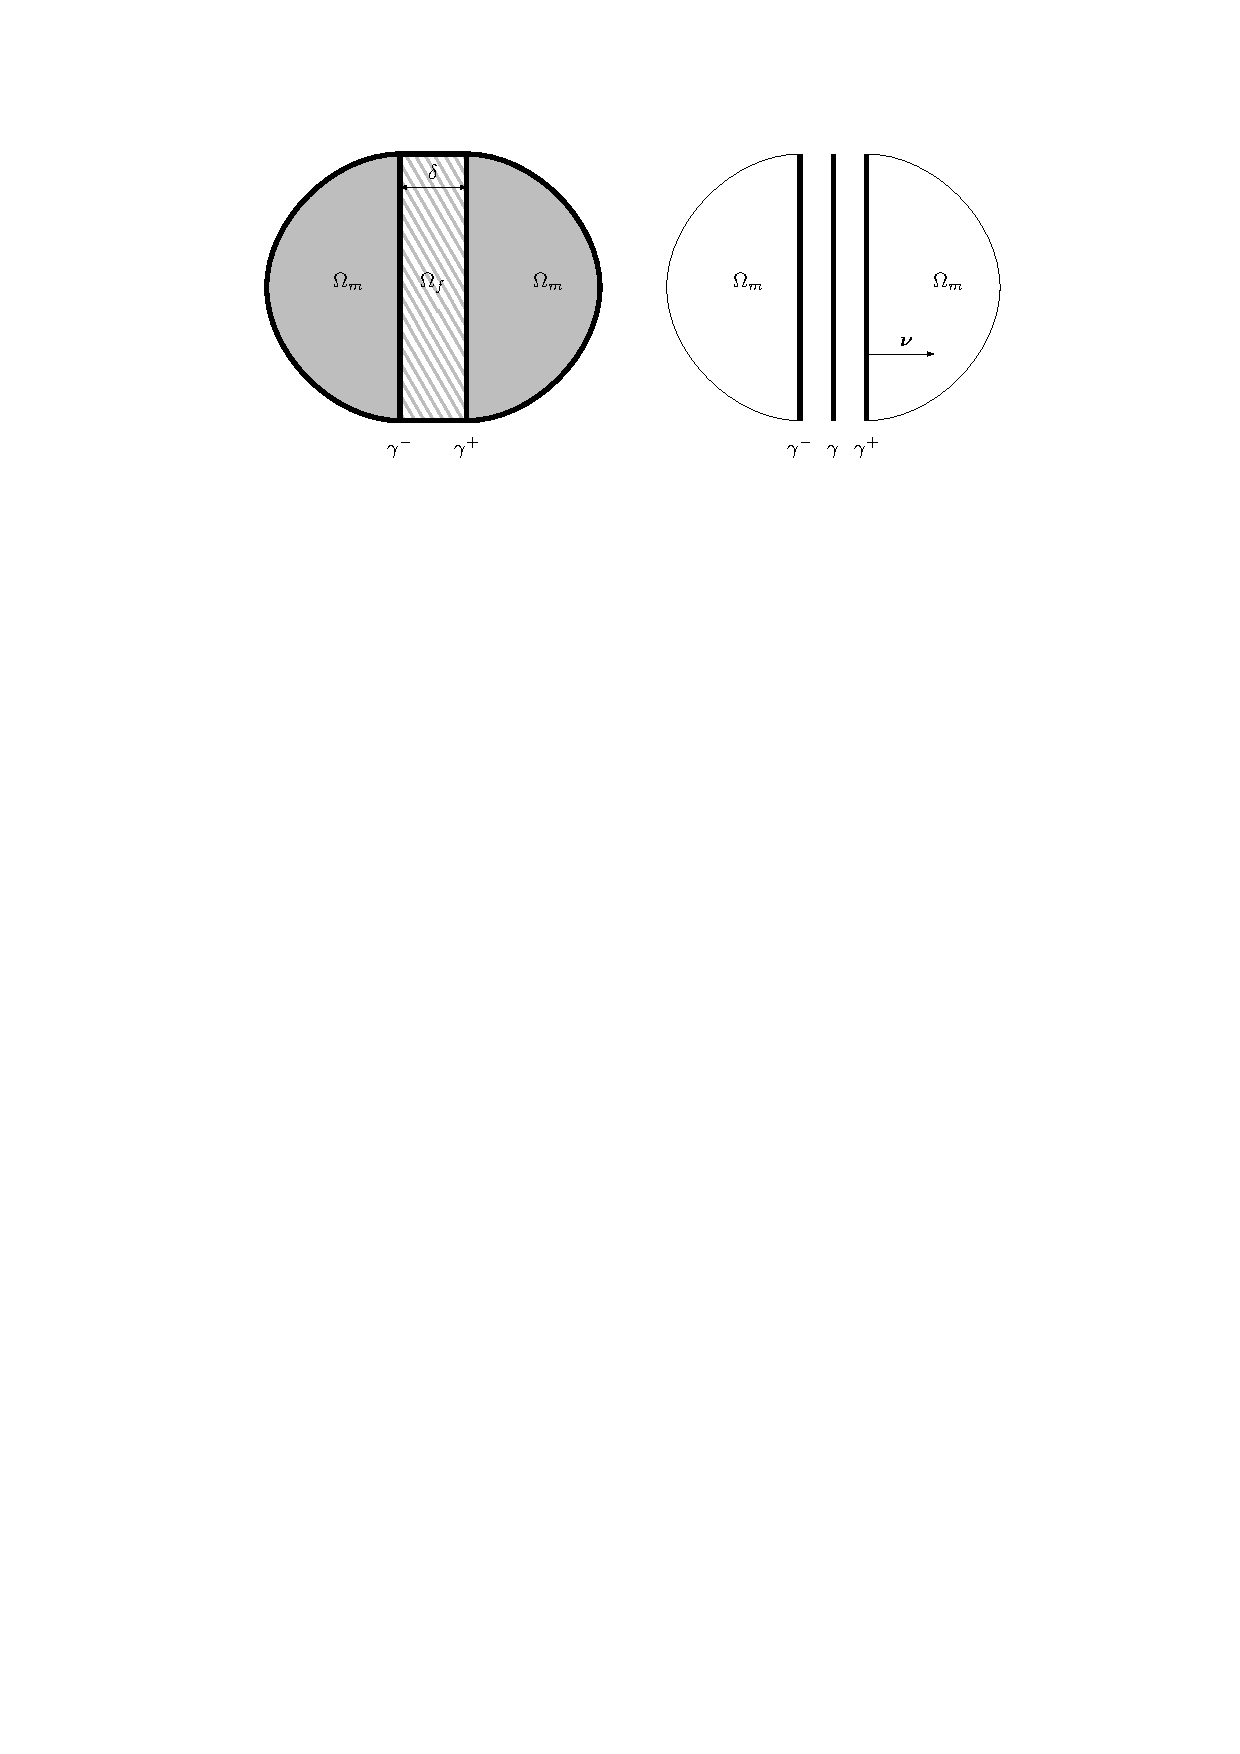
\includegraphics[width=\textwidth]{figures/omegas}
\label{fig:omegas}
\caption{The domain of the full model (left) and the reduced geometry (right).}
\end{figure}

We consider a bounded domain $\Omega \subset \Real^d$, $d=2,3$ with a Lipschitz boundary, see Figure \ref{fig:omegas} left). The domain $\Omega$ contains 
a fracture $\Omega_f:=\Omega\cap \big((-\delta/2,\delta/2)\times\Real^{d-1}\big)$ 
with the aperture $\delta>0$ surrounded by the matrix domain $\Omega_m:=\Omega\setminus\overline\Omega_f$. 
The left and right part of $\Omega_m$ will be denoted by $\Omega_{1}$ and $\Omega_{2}$, respectively.
% \note{JB}{$\Omega_m$ is not simply connected, thus not domain; are there some important consequences?}
The fracture interacts with the matrix domain on the interfaces 
$\gamma_1:=\Omega\cap\big( \{-\delta/2\}\times \Real^{d-1}\big)$ and 
$\gamma_2:=\Omega\cap\big( \{ \delta/2\}\times \Real^{d-1}\big)$. Normal vectors of these interfaces are denoted $\vc n_i$, $i=1,2$ with orientation out of the domain $\Omega_m$.
Further, we introduce reduced geometry (see Figure \ref{fig:omegas})
where the fracture domain is represented by the interface $\gamma:=\Omega\cap\big(\{0\}\times\Real^{d-1}\big)$ in its center. 

We shall derive a model of poroelasticity on the reduced geometry.
The starting point is the Biot system:
\begin{subequations}
\label{eq:biot}
\begin{align}
    \label{eq:lin_el}
    -\div \bbsigma_i &= \ff_i &&\mbox{ in }\Omega_i, ~i=1,2,f,\\
\label{eq:biot_darcy}    \prtl_t\left(\frac{p_i}{M_i} + \div(\alpha_i\uu_i)\right)-\div(\tn K_i\nabla p_i) &= g_i &&\mbox{ in }\Omega_i, ~i=1,2,f,
\end{align}
\end{subequations}
where
\[ \bbsigma_i = \bbsigma_i[\uu_i,p_i] = \tn C_i\ep[\uu_i]-\alpha_i p_i\tn I,~\ep[\uu_i]=\frac12(\nabla\uu_i+\nabla^\top\uu_i),~i=1,2,f. \]
The interface conditions between $\Omega_m$ and $\Omega_f$ are:
\[ \left.\begin{aligned}
p_i &= p_f\\
(\tn K_i\nabla p_i)\nn_i &= (\tn K_f\nabla p_f)\nn_i\\
\uu_i &= \uu_f\\
\bbsigma_i\nn_i &= \bbsigma_f\nn_i
\end{aligned} \right\} \mbox{ on }\gamma_i,~i=1,2. \]




\section{Calculus on the reduced fracture}

% For the sake of simplicity, we will not write subscript $f$ for quantities on the fracture. 
We set $\nn:=\nn_1$ and define
\[ \tn P := \nn\otimes\nn, \quad \kappa:=\div\nn \]
the projector onto the direction of $\nn$ and the mean curvature of $\gamma$ (so that $d/\kappa$ is the radius of the tangent ball).
We shall assume that
\[ \delta<2d/\kappa, \]
i.e. the fracture width is sufficiently small for large mean curvature.
Consequently, for any point $\xx\in\Omega_f$ there is a unique projection $\xx_\gamma\in\gamma$ such that
\[ \xx = \xx_\gamma \pm \dist(\xx,\gamma)\nn. \]
% By $x$, $\vc y$, we denote the normal and the tangential coordinate of a point in $\Omega_f$.

We shall decompose vectors and tensors into the normal and tangential parts:
\[ \begin{aligned}
\vv &= v_\nu\nn + \vv_\tau,\\
v_\nu &:= \vv\cdot\nn,\\
\vv_\tau &:= \vv-v_\nu\nn,\\
\tn A &= \tn A_\nu + \tn A_\tau,\\
\tn A_\nu &:= \tn A\tn P,\\
\tn A_\tau &:= \tn A-\tn A_\nu = \tn A(\tn I-\tn P).
\end{aligned} \]
For a vector-valued function $\vv$ we define the normal derivative:
\[ \prtl_\nu\vv := (\nabla\vv)\nn. \]
The normal and tangential part of the gradient of $\vv$ is then
\[ \begin{aligned}
\nabla_\nu\vv &:= (\nabla\vv)_\nu = \nabla\vv\tn P = \nn\otimes(\prtl_\nu\vv),\\
\nabla_\tau\vv &:= (\nabla\vv)_\tau.
\end{aligned} \]
The divergence of $\vv$ is decomposed into the normal and tangential part and an extra term due to the curvature of $\gamma$:
\begin{align}
\label{eq:div_v_split}\div\vv &= \div_\nu\vv + \div_\tau\vv + v_\nu\kappa,\\
\div_\nu\vv &:= \tn I:\nabla_\nu\vv = \tn P:\nabla\vv = (\prtl_\nu\vv)_\nu,\\
\div_\tau\vv &:= \div(\vv_\tau).
\end{align}
For a tensor-valued function $\tn A$ we split the divergence to the normal and tangentiald part:
\begin{subequations}
\label{eq:div_tn}
\begin{align}
\div\tn A &:= \div_\nu\tn A + \div_\tau\tn A,\\
\div_\nu\tn A &:= \div(\tn P\tn A)=\prtl_\nu(\tn A^\top\nn)+\kappa\tn A^\top\nn,\\
\div_\tau\tn A &:= \div((\tn I-\tn P)\tn A).
\end{align}
\end{subequations}
Let $w$ be a function defined in $\Omega_f$.
We denote its jump
\[ \jmp{w}(\xx) := w(\xx+\delta/2)-w(\xx-\delta/2),~\xx\in\gamma. \]
Accordingly, we shall use the following notation of jumps of the solutions and the fluxes:
\[ \jmp{p} := p_{2|\gamma_2}-p_{1|\gamma_1}, \]
\[ \jmp{\uu} := \uu_{2|\gamma_2}-\uu_{1|\gamma_1}, \]
\[ \jmp{\tn K\nabla p\cdot\nn} := (\tn K_2\nabla p_2\cdot\nn_2)_{|\gamma_2} + (\tn K_1\nabla p_1\nn_1)_{|\gamma_1}, \]
\[ \jmp{\bbsigma\nn} := (\bbsigma_2\nn_2)_{|\gamma_2} + (\bbsigma_1\nn_1)_{|\gamma_1}. \]
When integrating across the fracture, we shall write
\[ \int w\dn := \int w(\cdot+s\nn)\d s. \]
The symbol $\overline w$ will denote the integral mean of a function $w$ across the fracture aperture, i.e.
\[ \overline w(\vc x):=\frac1\delta\int_{-\delta/2}^{\delta/2} w \dn,~\vc x\in\gamma. \]
Then it holds:
\eq{ \label{eq:int_div_n}
\int_{-\delta/2}^{\delta/2}\prtl_\nu\vv\dn = \int_{-\delta/2}^{\delta/2}\frac{\rm d}{{\rm d}s}\left(\vv(\cdot+s\nn)\right)\d s = \jmp{\vv},
}
\[ \int_{-\delta/2}^{\delta/2}\nabla_\nu\vv\dn = \int_{-\delta/2}^{\delta/2}\nn\otimes(\prtl_\nu\vv)\dn
= \nn\otimes\jmp{\vv}. \]




\section{Continuum-fracture model for flow}

We assume that the parameters $M_f$, $\alpha_f$, $\tn K_f$ depend only on $\xx_\gamma$ \sout{and $\tn P\tn K=\tn P\tn K\tn P$} in $\Omega_f$.
The equation for $\overline p_f$ will be obtained from \eqref{eq:biot_darcy} by averaging and using the approximations
\eq{ \label{eq:approx_p} \nabla_\nu p_{i|\gamma_i} \approx \frac2\delta(\overline p_f-p_{i|\gamma_i})\nn_i,\quad \nabla_\tau p_{i|\gamma_i}\approx \nabla_\tau\overline p_f. }
Let us integrate \eqref{eq:biot_darcy} over the fracture aperture.
We get:
\eq{ \label{eq:darcy_int} \prtl_t\left(\frac\delta{M_f}\overline p_f + \int_{-\delta/2}^{\delta/2}\div(\alpha_f\uu_f)\d\nn\right)-\int_{-\delta/2}^{\delta/2}\div(\tn K_f\nabla p_f)\d\nn = \delta\overline g_f \mbox{ in }\gamma. }
The first integral in \eqref{eq:darcy_int} will be rewritten using \eqref{eq:div_v_split} and \eqref{eq:int_div_n}:
\ml{ \int_{-\delta/2}^{\delta/2}\div(\alpha_f\uu_f)\d\nn = \int_{-\delta/2}^{\delta/2}\div_\tau(\alpha_f\uu_f)\d\nn + \int_{-\delta/2}^{\delta/2}\div_\nu(\alpha_f\uu_f)\d\nn\\
+ \kappa\int_{-\delta/2}^{\delta/2}\alpha_f u_{f\nu}\d\nn
= \div_\tau(\delta\alpha_f\overline\uu_f) + \alpha_f(\jmp{\uu} + \kappa\overline\uu_f)\cdot\nn. }
% 
Before we rewrite the second integral in \eqref{eq:darcy_int} we approximate the flux on $\gamma_i$, $i=1,2$ usig \eqref{eq:approx_p}:
\ml{ \label{eq:approx_flux_gamma_i} \tn K_f\nabla p_{f|\gamma_i}\cdot\nn_i = \tn K_f(\nabla_\nu p_{f|\gamma_i} + \nabla_\tau p_{f|\gamma_i})\cdot\nn_i\\
\approx \tn K_f\left(\frac2\delta(\overline p_f-p_{i|\gamma_i})\nn_i + \nabla_\tau\overline p_f\right)\cdot\nn_i =: F_i. }
Then we can split the second integral in \eqref{eq:darcy_int} as follows:
\ml{ \int_{-\delta/2}^{\delta/2}\div(\tn K_f\nabla p_f)\d\nn = \int_{-\delta/2}^{\delta/2}\div_\nu(\tn K_f\nabla p_f)\d\nn + \int_{-\delta/2}^{\delta/2}\div_\tau(\tn K_f\nabla p_f)\d\nn\\
+ \kappa\int_{-\delta/2}^{\delta/2}(\tn K_f\nabla p_f)_\nu\d\nn }
and treat each term separately using \eqref{eq:int_div_n} and \eqref{eq:approx_flux_gamma_i}:
\eq{ \int_{-\delta/2}^{\delta/2}\div_\nu(\tn K_f\nabla p_f) = \tn K_f\jmp{\nabla p}\cdot\nn = -\sum_{i=1}^2\tn K_f\nabla p_{f|\gamma_i}\cdot\nn_i
\approx  -\sum_{i=1}^2 F_i, }
% 
\ml{ \int_{-\delta/2}^{\delta/2}\div_\tau(\tn K_f\nabla p_f) = \int_{-\delta/2}^{\delta/2}\div_\tau(\tn K_f\nabla_\nu p_f) + \int_{-\delta/2}^{\delta/2}\div_\tau(\tn K_f\nabla_\tau p_f)\\
= \div_\tau(\tn K_f\nn\jmp{p}) + \div_\tau(\delta\tn K_f\nabla_\tau\overline p_f), }
% 
\ml{ \label{eq:darcy_int_kappa} \kappa\int_{-\delta/2}^{\delta/2}(\tn K_f\nabla p_f)_\nu = \kappa\int_{-\delta/2}^{\delta/2}(\tn K_f\nabla_\nu p_f)\cdot\nn + \kappa\int_{-\delta/2}^{\delta/2}(\tn K_f\nabla_\tau p_f)\cdot\nn\\
= \kappa\left( \tn K_f\nn\cdot\nn\jmp{p} + \tn K_f\nabla_\tau\overline p_f\cdot\nn \right). }
From \eqref{eq:darcy_int}-\eqref{eq:darcy_int_kappa} we obtain the flow equation in the reduced fracture:
\eq{ \prtl_t\left(\frac\delta{M_f}\overline p_f + \div_\tau(\delta\alpha_f\overline\uu_f)\right)-\div_\tau(\delta\tn K_f\nabla_\tau\overline p_f) - \sum_{i=1}^2F_i + G = \delta \overline g_f \mbox{ in }\gamma, }
where
% \[ F_i = \tn K_f\left(\frac2\delta(\overline p_f-p_{i|\gamma_i})\nn_i + \nabla_\tau\overline p_f\right)\cdot\nn_i, ~i=1,2, \]
\[ G = \prtl_t\left(\alpha_f(\jmp{\uu} + \kappa\overline\uu_f)\cdot\nn\right) -\div_\tau(\tn K_f\nn\jmp{p}) - \kappa\tn K_f\nn\cdot\nn\jmp{p} - \kappa\tn K_f\nabla_\tau\overline p_f\cdot\nn. \]
The interface condition on $\gamma_i$, $i=1,2$ becomes
\eq{ (\tn K_i\nabla p_i)_{|\gamma_i}\cdot\nn_i = F_i. }





\section{Continuum-fracture model for elasticity}
% \label{sc:ad_on_fractures}

In this section, we shall integrate the equation \eqref{eq:lin_el} across the fracture and obtain its approximation on the surface $\gamma$ running through the middle of the fracture.
We assume that 
\[ \forall\xx\in\Omega_f:~\tn C_f(\xx)=\tn C_f(\xx_\gamma), \]
i.e. $\tn C_f$ is constant in the normal direction of $\Omega_f$.
Further we assume the usual symmetries of $\tn C_i$, $i=1,2,f$, i.e.
\[ \forall k,l,m,n=1,\ldots,d:~ [\tn C_i]_{klmn}=[\tn C_i]_{lkmn}=[\tn C_i]_{klnm}=[\tn C_i]_{mnkl}. \]
% In order to make the procedure mathematically correct, we have to assume that the functions
% $\prtl_\nu w$, $\prtl_\nu \grad_{\vc y} u$, $\prtl_\nu \vc b_{\vc y}$ are continuous and bounded on $\Omega_f$, moreover
Using the identity \eqref{eq:div_tn} we decompose the term on the left hand side of \eqref{eq:lin_el} as follows:
\begin{equation}
\label{eq:decomp_div_sigma}
\div\bbsigma_f = \prtl_\nu(\bbsigma_f\nn) + \kappa\bbsigma_f\nn\\
+ \div_\tau(\tn C_f\nabla_\tau\uu_f - \alpha_f p_f\tn I)
+ \div_\tau(\tn C_f\nabla_\nu\uu_f).
\end{equation}
Integrating \eqref{eq:decomp_div_sigma} over the fracture aperture we obtain:
\begin{equation}
    \label{eq:integrate_div_sigma}
   \int_{-\delta/2}^{\delta/2}\div\bbsigma_f\dn
   = -\jmp{\bbsigma\nn}
   + \kappa\vc S
   + \div_\tau(\delta\bbsigma^\tau) + \vc R,
\end{equation}
where
\[ \bbsigma^\tau = \bbsigma^\tau[\overline\uu_f,\overline p_f] := \tn C_f\nabla_\tau\overline\uu_f - \alpha_f \overline p_f\tn I_\tau, \]
\[ \vc S = \vc S[\uu_1,\uu_2,\overline\uu_f,\overline p_f] := \delta\bbsigma^\tau\nn + \tn C_f(\jmp{\uu}\otimes\nn), \]
\[ \vc R = \vc R[\uu_1,\uu_2]=\div_\tau(\tn C_f(\jmp{\uu}\otimes\nn)), ~i=1,2. \]
% $\uu_f:=\overline\uu$, $p_f:=\overline p$, $\uu_i:=\uu_{|\Omega_{mi}}$ and $p_i:=p_{|\Omega_{mi}}$, $i=1,2$.
We shall approximate the normal part of the gradient of $\uu_f$ at the interface $\gamma_i$, $i=1,2$, using the integral mean over one half of the fracture:
\ml{ \nabla_\nu\uu_{f|\gamma_i} \approx \frac2\delta\int_{(i-2)\frac\delta2}^{(i-1)\frac\delta2}\nabla_\nu\uu_f\,\dn
= \frac2\delta\left(\uu_{f|\gamma}-\uu_{f|\gamma_i}\right)\otimes\nn_i\\
\approx \frac2\delta\left(\overline\uu_f-\uu_{i|\gamma_i}\right)\otimes\nn_i =: \mathbb\Phi_i,~i=1,2. }
Then we have:
\eq{ \int_{-\delta/2}^{\delta/2} \nabla_\nu\uu_f\dn = \jmp{\uu}\otimes\nn = \frac\delta2(\mathbb\Phi_1 + \mathbb\Phi_2). }
The tangential part of the gradient of $\uu_f$ will be approximated as follows:
\[ \nabla_\tau\uu_{f|\gamma_i} \approx \nabla_\tau\overline\uu_f. \]
The normal stress at $\gamma_i$, $i=1,2$ will be approximated as follows:
\ml{
\label{eq:approx_sigma_flux}
(\bbsigma_f\nn_i)_{|\gamma_i} = \tn C_f(\nabla_\nu\uu_{f|\gamma_i}+\nabla_\tau\uu_{f|\gamma_i})\nn_i - \alpha_f p_{i|\gamma_i}\nn_i\\
\approx \left(\tn C_f(\mathbb\Phi_i + \nabla_\tau\overline\uu_f)\right)\nn_i - \alpha_f p_{i|\gamma_i}\nn_i =: \mathbb\Sigma_i. }
% where
% \begin{multline}
% \frac2\delta\int_0^{\delta/2}\tn C(\nabla\uu)\nn_2 = \frac2\delta\int_0^{\delta/2}\left(\tn C(\nabla_\tau\uu)+\tn C(\nabla_\nu\uu)\right)\nn_2~dx\\
% \approx \tn C(\nabla_\tau\uu_f)\nn_2 + \frac2\delta\tn C((\uu_f-\uu_2)\otimes\nn_2)\nn_2.
% \end{multline}
% Similarly we get
% \begin{equation}
% \label{eq:integrate_sigma_flux_1}
% \tn C(\nabla\uu_1)\nn_1 \approx \tn C(\nabla_\tau\uu_f)\nn_1 + \frac2\delta\tn C((\uu_f-\uu_1)\otimes\nn_1)\nn_1.
% \end{equation}
% Hence
% \[ \bbsigma_i\nn_i \approx \vc Q_i[\uu_i,\uu_f,p_i] := \tn C(\nabla_\tau\uu_f)\nn_i + \frac2\delta\tn C((\uu_f-\uu_i)\otimes\nn_i)\nn_i - \alpha p_i\nn_i. \]
Consequently, we obtain from \eqref{eq:lin_el} and \eqref{eq:decomp_div_sigma}--\eqref{eq:approx_sigma_flux} the continuum-fracture system for linear elasticity:
\[ \begin{aligned}
-\div_\tau(\delta\bbsigma^\tau) - \sum_{i=1}^2\tn\Sigma_i - \vc R - \kappa\vc S &= \delta\overline\ff &&\mbox{ in }\gamma, \\
-\div\bbsigma_i &= \ff &&\mbox{ in }\Omega_{i}, ~i=1,2,\\
\bbsigma_i\nn_i &= \vc Q_i &&\mbox{ on }\gamma_i,~i=1,2. \end{aligned} \]





\section{Mixed formulation for incompressible elastic material}
TOHLE JE ZATIM JEN PRO ROVINNE PUKLINY

In this section we shall assume that the elasticity tensor has the form
\[ c_{ijkl} = \mu(\delta_{ik}\delta_{jl} + \delta_{il}\delta_{jk}) + \lambda\delta_{ij}\delta_{kl}, ~i,j,k,l=1,...,d, \]
and hence
\[ \vc\sigma[\uu,p] = 2\mu\ep[\uu] + (\lambda\div\uu - \alpha p)\tn I. \]
Further we shall assume that the material parameter $\alpha$ is constant in $\Omega_{mi}$, $i=1,2$ and in $\gamma$.
We aim to derive a formulation which is suitable for the incompressible case, i.e. when $\lambda\to\infty$.
For this reason we introduce a new quantity
\[ \phi:=\alpha p-\lambda\div\uu, \]
so that the stress tensor becomes
\[ \vc\sigma=\vc\sigma[\uu,\phi] = 2\mu\ep[\uu] - \phi\tn I. \]
The Biot system in the matrix domain now reads:
\[ \left.\begin{aligned}
-\div(2\mu\ep[\uu_i]) + \nabla\phi_i &= \ff\\
\prtl_t\left(\left(\frac1M+\frac{\alpha^2}\lambda\right)p_i - \frac\alpha\lambda\phi_i\right)-\div(\tn K\nabla p_i) &= g\\
\div\uu_i - \frac\alpha\lambda p_i + \frac1\lambda\phi_i &= 0
\end{aligned}\right\} \mbox{ in }\Omega_{mi}, ~i=1,2. \]
After integrating across the fracture we obtain:
% The continuum-fracture system for poroelasticity now reads:
\[ \left.\begin{aligned}
-\div_\tau(2\delta\mu\ep_\tau[\uu_f]) + \nabla_\tau(\delta\phi_f) + \sum_{i=1}^2\tilde{\vc Q}_i + \tilde{\vc R} &= \delta\overline\ff\\
\prtl_t\left(\delta\left(\frac1M+\frac{\alpha^2}\lambda\right) p_f - \delta\frac\alpha\lambda\phi_f\right)-\div_\tau(\delta\tn K\nabla_\tau p_f)  + \sum_{i=1}^2F_i &= \delta \overline g\\
\div_\tau(\delta\uu_f) + \sum_{i=1}^2(\uu_f-\uu_i)\cdot\nn_i - \delta\frac\alpha\lambda p_f + \frac\delta\lambda\phi_f &= 0
\end{aligned} \right\} \mbox{ in }\gamma, \]
with the interface conditions
\[ \left.\begin{aligned}
\vc\sigma[\uu_i,\phi_i]\nn_i &= \tilde{\vc Q}_i \\
\tn K\nabla p_i\nn_i &= F_i \end{aligned} \right\} \mbox{ on }\gamma_i,~i=1,2, \]
where
\[ \begin{aligned}
\tilde{\vc Q}_i &= 2\mu\ep_\tau[\uu_f]\nn_i + \frac4\delta\mu(\uu_f-\uu_i) - \phi_f\nn_i, \\
\tilde{\vc R} &= \sum_{i=1}^2\div_\tau(\mu(\uu_i\otimes\nn_i+\nn_i\otimes\uu_i)). \end{aligned} \]
One can notice that in the limit $\lambda\to\infty$, the flow and elasticity become independent.



\bibliographystyle{abbrvnat}
\bibliography{flow123d_doc.bib}
%%%%%%%%%%%%%%%%%%%%%%%%%%%%%%%%%%%%%%%%%%%%%%%%%%%%%%%%%%%%%%%%%%%%%%%%%%%%%%%%%%%%%%%%%%%%%%%%%%%%%%%%%%%%%%%%%


\end{document}


